\chapter{Appendix E: Supporting SADb Records}\label{app:sadb_records}
\graphicspath{{../Figures/96-AppendixE/}{figs/96-AppendixE/}}

This appendix records the curation snapshot and pathway examples supporting Chapter~\ref{ch:database}. Counts refer to the stated audited or retained set; they are not estimates of the size of the neuroscience literature.

\section{Record Sets and Coverage}

The application contains 1,393 records from the five-table base: 943 Papers, 247 Models, 157 Review Papers, 42 Feedback pathways, and 4 Recorders. Of these, 436 are in the app but not in Airtable due to their 1000 entry limitation. The retained working base in Airtable contains 957 records: 561 Papers, 244 Models, 109 Review Papers, 39 Feedback pathways, and 4 Recorders. The application table includes all record types, while its pivot and citation views use the paper set.

Coverage of the application's Papers category is reported in Chapter~\ref{ch:database}: among its 943 entries, 833 have curation notes, 606 preparation tags, 316 animal-study assessments, 119 pathway links, 95 afferent classifications, 363 robot/simulation translation notes, 892 DOIs, and 318 attached-PDF indicators. The following retained-set counts describe the maintenance subset only and use a different denominator.

Among the 561 retained papers, 523 carry curation notes, 426 preparation tags, 240 notes assessing animal-study potential, 118 links to named feedback pathways, 86 an afferent classification, and 258 robot/simulation translation notes. There are 550 DOIs; 38 records remain without grounding text. These fields overlap and should not be summed as disjoint categories.

The citation graph covers the 943-paper audit: 730 connected papers, 11,130 directed in-corpus citation pairs, and 18 Louvain groups. Citation proximity is a navigation aid, not mechanistic evidence. Chapter~\ref{ch:database} shows the citation view (Figure~\ref{fig:sadb_clusters}); Figure~\ref{fig:sadb_explorer} shows the paper table.

\begin{figure}[htbp]
\centering
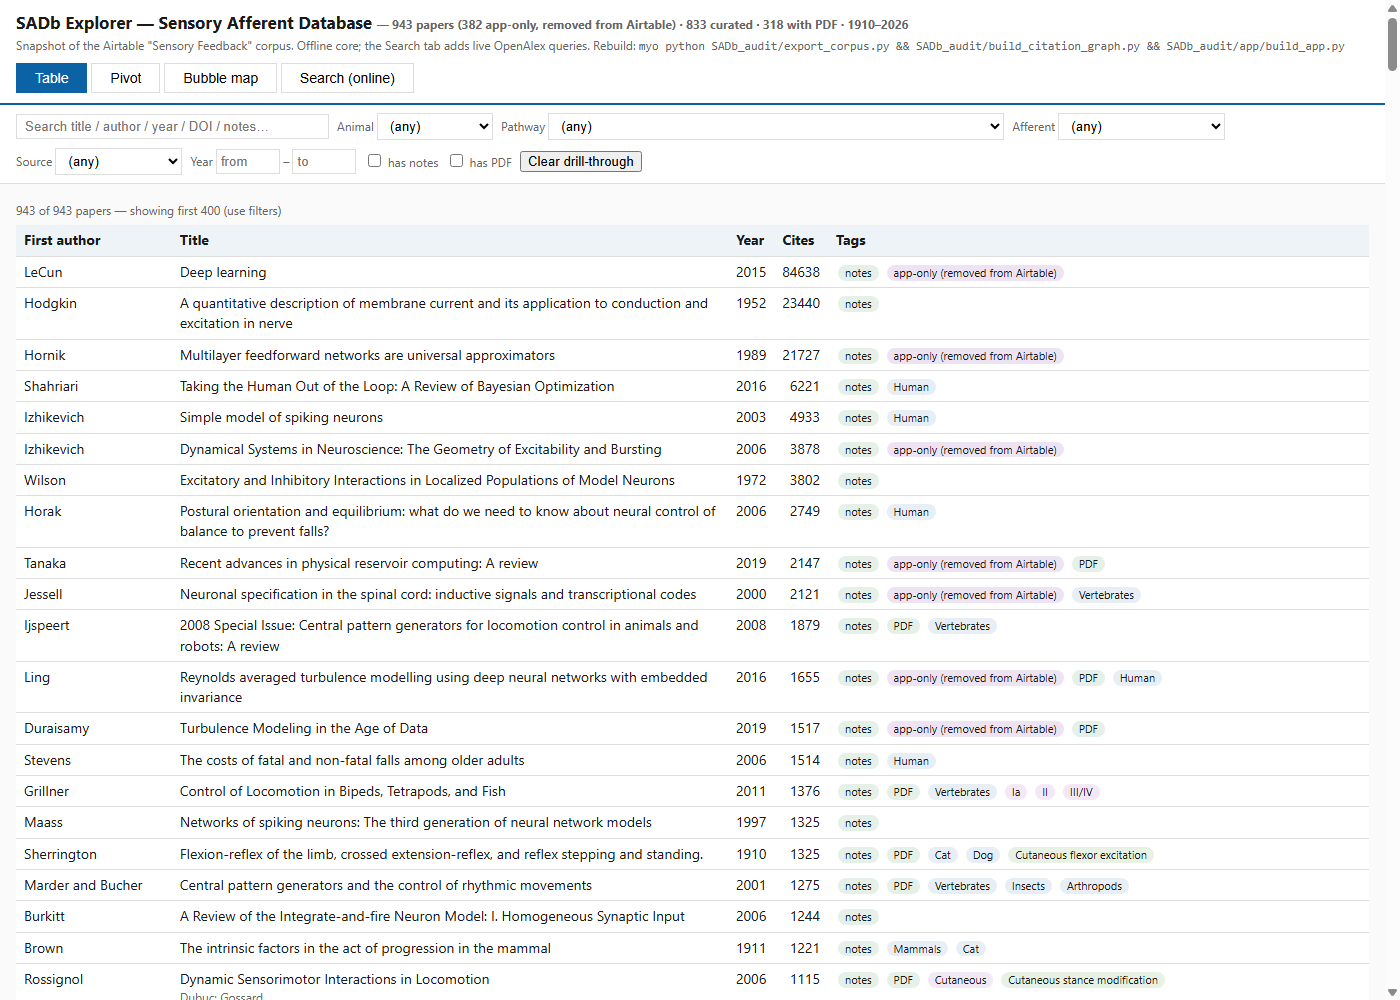
\includegraphics[width=\textwidth]{sadb_explorer.png}
\caption[The SADb Explorer]{SADb Explorer paper-table view. Searches and filters expose bibliographic information, curation notes, preparation tags, and afferent or pathway links. The embedded corpus is available offline.}
\label{fig:sadb_explorer}
\end{figure}

\section{Afferent Classes and Linked Pathways}

The tables reproduce the curated signal summaries and representative linked pathways. Their record names are database labels; pathway action depends on the experimental preparation and locomotor state described in the cited sources. Translating these records into a controller requires an explicit encoding and verification step.

\begin{table}[htbp]
\caption{Afferent classes, encoded signals, and pathway roles represented in the Sensory Afferent Database. References link to corpus records; Ia, II, and Ib signal summaries follow \citet{prochazka_ensemble_1998}.}
\label{tab:sadb_afferents}
\small
\begin{tabularx}{\textwidth}{@{}>{\raggedright\arraybackslash}p{0.14\textwidth}>{\raggedright\arraybackslash}p{0.16\textwidth}>{\raggedright\arraybackslash}p{0.16\textwidth}>{\raggedright\arraybackslash}X@{}}
\toprule
\textbf{Class} & \textbf{Receptor} & \textbf{Signal carried} & \textbf{Recorded pathway roles (anchors)} \\
\midrule
Ia & muscle spindle primary & muscle length and velocity & homonymous stretch excitation \citep{eccles_integrative_1958}; reciprocal inhibition of the antagonist pool \citep{jankowska_effect_1967} \\
II & muscle spindle secondary & static muscle length & midlumbar disynaptic relay onto motor nuclei \citep{edgley_interneuronal_1987}; stance-phase support of extensor activity \citep{mazzaro_afferent_2006} \\
Ib & Golgi tendon organ & whole-muscle force & autogenic inhibition at rest, stance-phase reversal to excitation, and the load gate on swing onset \citep{dietz_significance_2000, dominguez_candidate_2020} \\
III/IV & free nerve endings & metabolic and nociceptive signals, converging with cutaneous and group II--III afferents as flexor-reflex afferents & phase-dependent resetting of the locomotor rhythm \citep{schomburg_flexor_1998} \\
Cutaneous & skin and foot-pad receptors & contact and perturbation events & flexor excitation and phase-modulated stance correction \citep{sherrington_flexion_1910, forssberg_stumbling_1979} \\
\bottomrule
\end{tabularx}
\end{table}

\begin{sidewaystable}[p]
\caption{Principal feedback pathways, named by afferent, action, and phase, with linked demonstrating papers. Counts are identical in the audited 943-paper corpus and retained 561-paper corpus.}
\label{tab:sadb_pathways}
\fontsize{10pt}{12pt}\selectfont
\begin{tabularx}{\textheight}{@{}llXrp{0.26\textheight}@{}}
\toprule
\textbf{Pathway record} & \textbf{Class} & \textbf{Recorded action in the step cycle} & \textbf{Linked papers} & \textbf{Demonstrating references} \\
\midrule
Ia monosynaptic excitation & Ia & stretch excitation of the homonymous motor pool, with the pathway gain modulated over the step cycle & 7 & \citep{eccles_integrative_1958, capaday_amplitude_1986} \\
Ia reciprocal inhibition & Ia & inhibition of the antagonist motor pool through the Ia inhibitory interneurons, rhythmically active in fictive locomotion & 6 & \citep{jankowska_effect_1967, pratt_ia_1987} \\
Ib disynaptic inhibition & Ib & autogenic non-reciprocal group I inhibition of the loaded muscle's own pool, reduced during stance & 5 & \citep{jankowska_common_1981, stephens_short_1996} \\
Ib disynaptic excitation & Ib & the locomotor reversal: group I input excites synergist extensor pools during the extensor phase, replacing the resting inhibition & 6 & \citep{mccrea_disynaptic_1995, pearson_enhancement_1998} \\
Ib stance to swing & Ib & the load gate: Ib input from ankle extensors prolongs stance, so swing is not initiated while the leg is loaded & 17 & \citep{dietz_significance_2000, dominguez_candidate_2020} \\
Ia or II stance to swing & Ia, II & flexor-length gate on stance termination: lengthening of flexor muscles in late stance ends extension and resets the cycle & 10 & \citep{hiebert_contribution_1996, akay_degradation_2014} \\
type II excitatory & II & stance-phase support of ankle-extensor activity through the midlumbar group II relay & 5 & \citep{edgley_interneuronal_1987, mazzaro_afferent_2006} \\
Cutaneous flexor excitation & Cutaneous & flexion withdrawal and the stumbling corrective reaction, phase-modulated over the cycle & 16 & \citep{sherrington_flexion_1910, forssberg_stumbling_1979} \\
\bottomrule
\end{tabularx}
\end{sidewaystable}
